\section{Methodology}
% Description of your proposed methodology or approach
In this section, we display how effective image preprocessing and our docking procedure collectively lead to a plausible method to train our model without manual labeling, which would be required, for our case, in real-world applications. Our methodology includes data collection, model training, inference, server integration, evaluation, and experimental setup.

\subsection{Data Collection}
We collect training data using a simulated environment created in a game engine \citep{hoster2024usinggameenginesmachine}. Our game engine of choice is Godot, a free and open source game engine. The environment consists of a robot and a docking station, with the robot's camera capturing images of the docking station from various angles. We then extract the coordinates of the targets using OpenCV, something that can only be done in the virtual world, as the real world does indeed have red and green in its colors, not just for the targets (as is used in the virtual world).
\begin{figure}
    \centering
    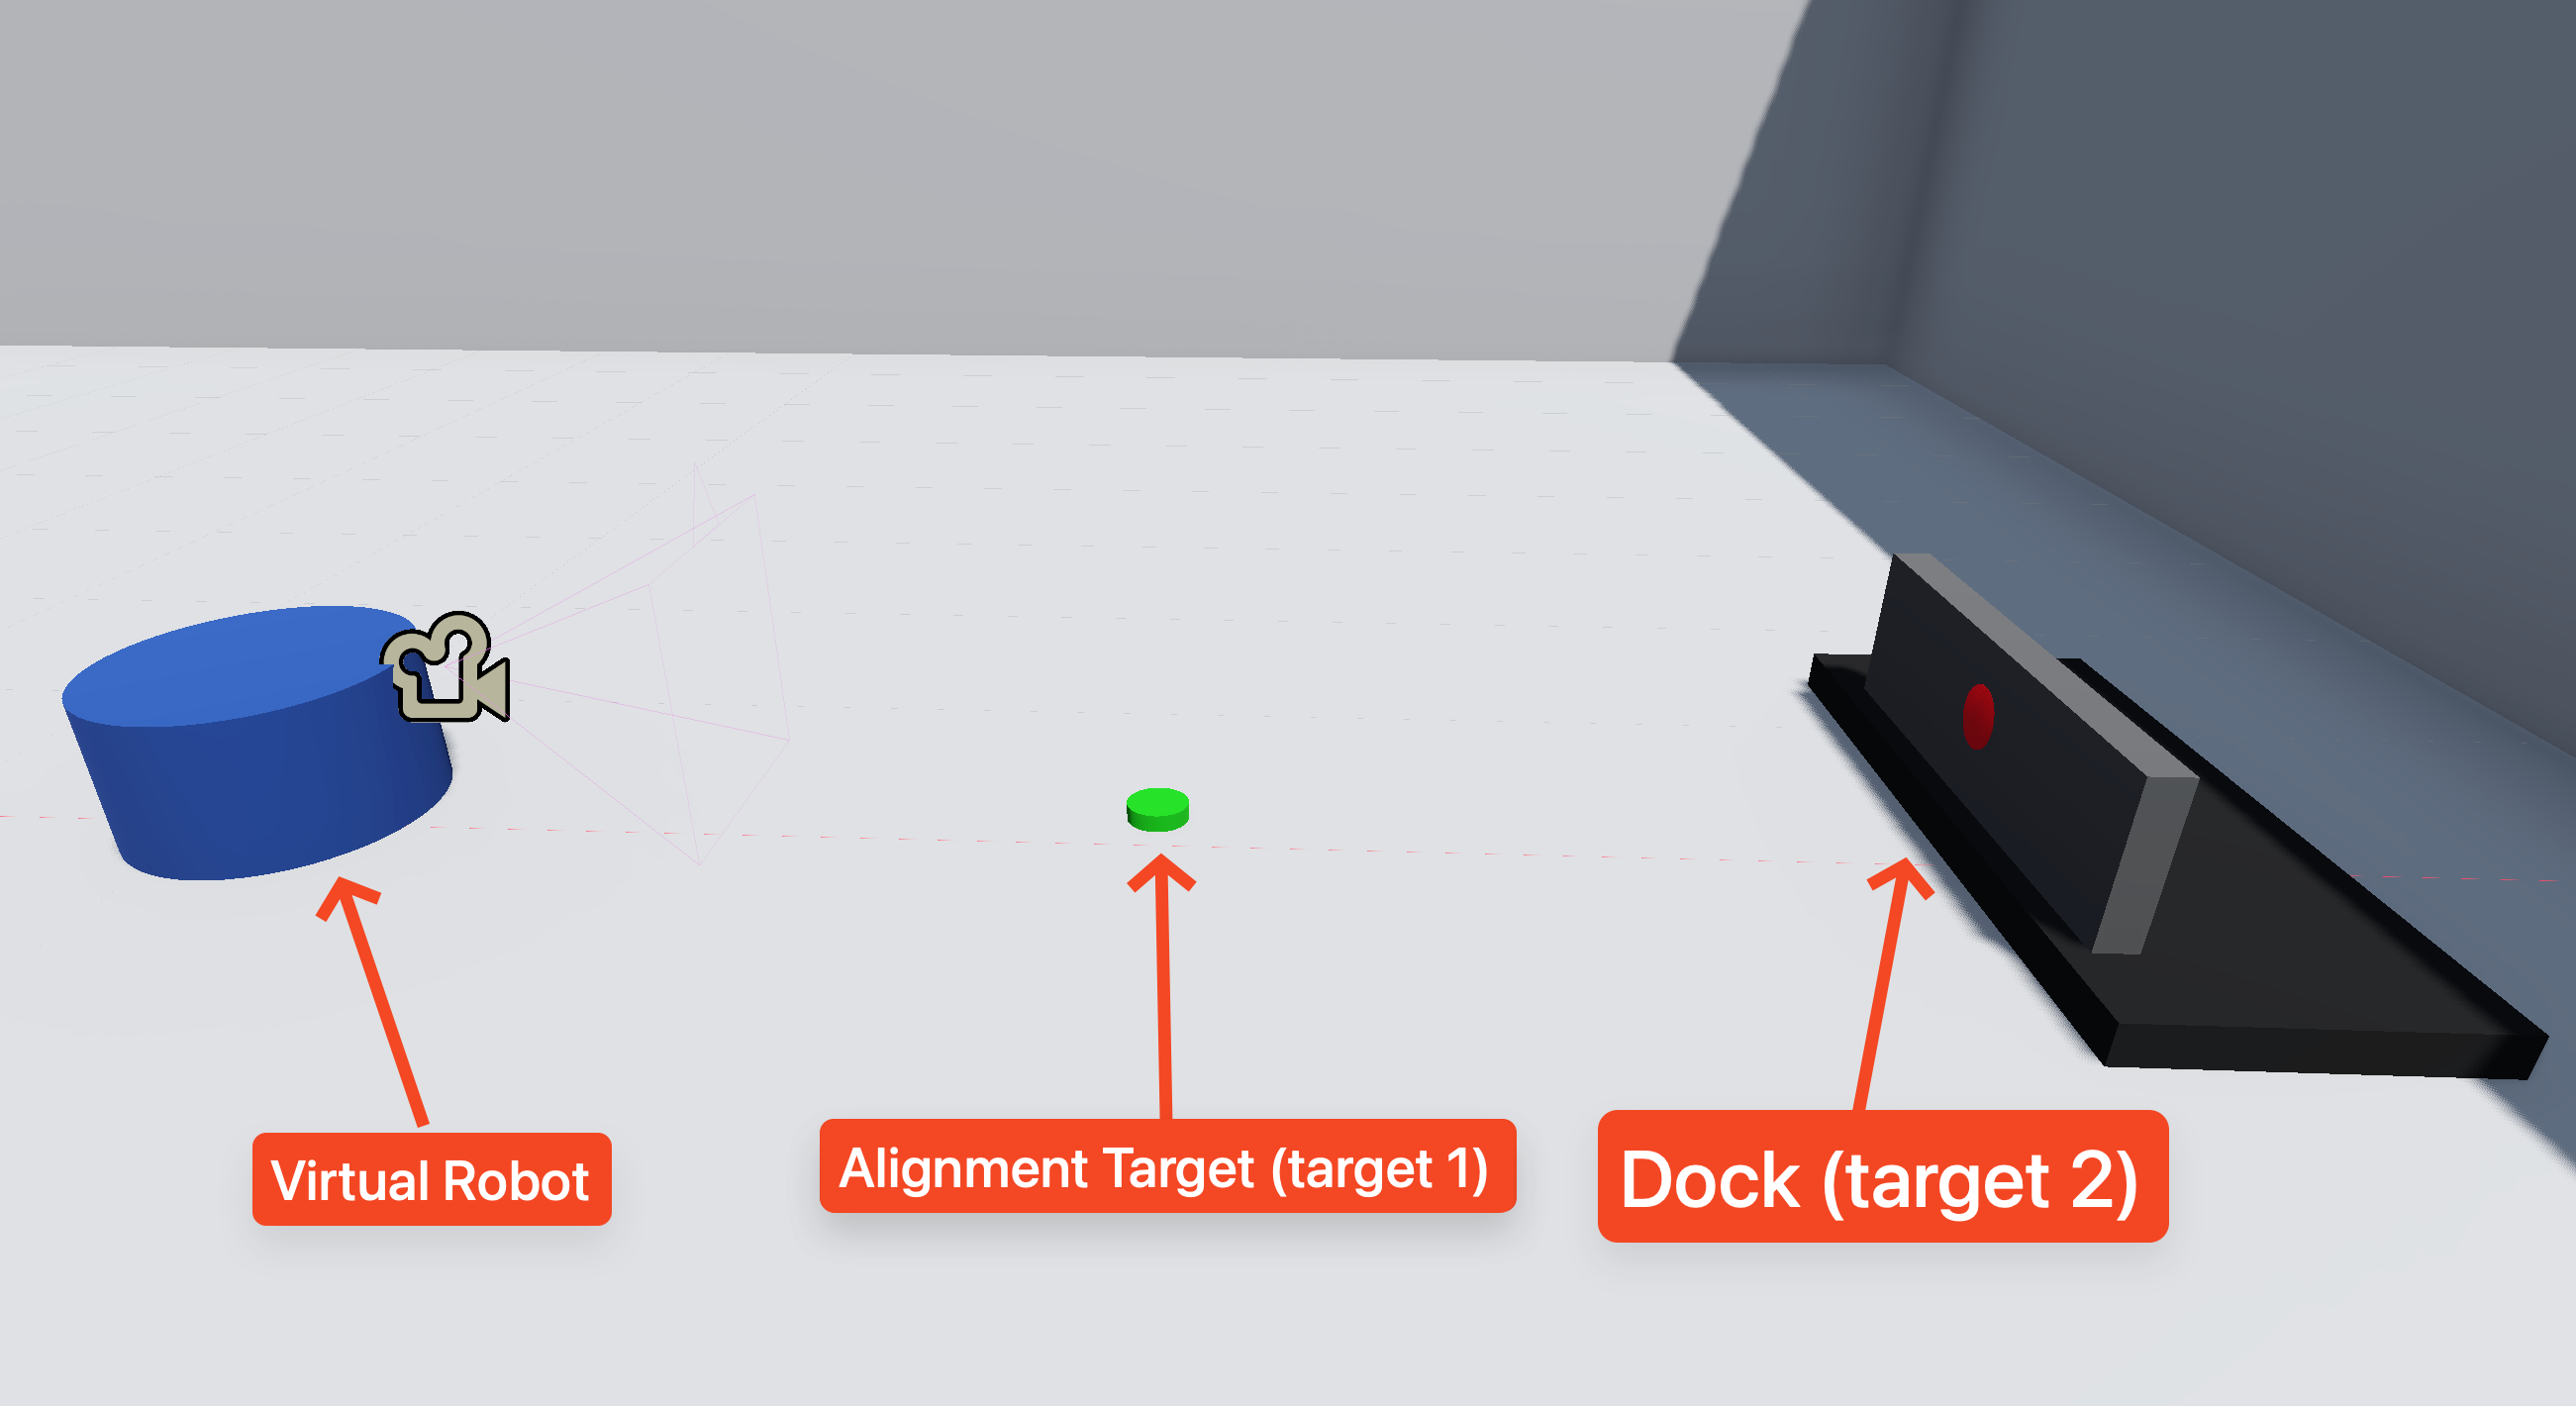
\includegraphics[width=\linewidth]{figures/src/virtual_world.png}
    \caption{
	    \textbf{Virtual world \& Labels} In our virtual world, we make targets 1 and 2 distinguishable from their surrounding environment by giving them a unique color.
    }
    \label{fig:virtual world}
\end{figure}


\subsection{Model Training}
% We train a deep learning model using PyTorch, as implemented in [src/machine_learning/model1/train.py](src/machine_learning/model1/train.py). The model architecture is defined in the `Predictor` class, and the training process involves the following steps:
\begin{enumerate}
    \item Load and preprocess the images using the `transforms` module from torchvision.
    \item Define the custom dataset class `TargetsDataset` to handle the input data.
    \item Instantiate the model, loss function (L1 Loss), and optimizer (Adam).
    \item Train the model over multiple epochs, adjusting the weights based on the loss calculated from the predicted and actual target values.
\end{enumerate}

\subsection{Inference}
For inference, we use the trained model to predict the next action based on a single input frame. The `predict` function takes an image as input, preprocesses it, and outputs the predicted target coordinates.

\subsection{Server Integration}
To facilitate real-time predictions, we can integrate the inference script with a Flask server, as shown in . The server receives images via POST requests, runs the inference, and returns the next action the virtual robot should take. This setup allows for seamless integration with other systems and real-time decision-making.

\subsection{Evaluation}
We evaluate the performance of our model using various metrics, including accuracy and loss values. The evaluation scripts are included in [tests/tests.py](tests/tests.py), which contain unit tests to ensure the correctness and robustness of our data processing and model training pipelines.

\subsection{Experimental Setup}
Our experimental setup involves running the training and inference scripts on a machine with a GPU to accelerate the deep learning computations. The models are saved in the [models](models) directory, and the results are analyzed and visualized using matplotlib.

\subsection{Conclusion}
Our methodology demonstrates a novel approach to robot docking using monocular vision and deep learning. By leveraging a simulated environment for data collection and a robust training pipeline, we achieve accurate and efficient docking without the need for additional sensors or reinforcement learning.
